% !TEX root = mythesis.tex

%==============================================================================
\chapter{Ultra High Energy Cosmic Rays and Neutrinos}
\label{sec:crneas}
%==============================================================================

\section{Ultra High Energy Cosmic Rays}
\label{sec:UHECR}
\subsection{History}
\label{subsec:crhist}
As already mentioned in the introduction cosmic rays have been a source of investigation for more than a century now. Even before the balloon flight by Victor Hess it was Henry Becquerel, the discoverer of radioactivity who believed that the \textit{atmospheric electricity}(ionization of air) was due to the radioactive substances present on Earth. In such a scenario the ionization rate should decrease the higher up you go in the atmosphere. The first measurements disproving this theory were performed by Theodor Wulf in 1909 with his own developed electrometer. His measurements published in the \textit{Physikalische Zeitschrift} indicated a higher level of radiation at the top of the Eiffel Tower as compared to its base. Unfortunately the measurements were not widely accepted, and it would take three years till Victor Hess via his several balloon flights provided irrefutable measurements corroborating Wulf's observations.

Between 1911-1912 Victor Hess performed nine(2 in 1911 and 7 in 1912) balloon flights going as high as 5350m a.s.l to measure the dependence of ionization rate to altitude. He carried with him three Wulf electrometers, two tuned for $\gamma$ rays and the third tuned for $\beta$ rays~\cite{}(1808.02927) which along with $\alpha$ were the only three known radioactive decays. His measurements published in the Proceedings of the Viennese Academy of Sciences~\cite{} showed that the radiation level decreased slightly up to a certain altitude (~1 km) but after this height the radiation increased significantly and at the highest flown altitudes reached levels about twice in comparison to the ones at sea level. Some of his measurements were done during the night and one during a partial solar eclipse which further made him rule out Sun as a source of this radiation. With further confirmations via the measurements by Werner Kolhörster in 1914 and Robert Millikan, in 1925, Victor Hess was awarded the Nobel Prize in Physics in 1936. 

Cosmic rays were still presumed to be gamma rays. This supposition was quickly negated by the efforts of Jacob Clay who via his measurements of the cosmic ray intensity at different latitudes by while sailing from Java to the Netherlands in 1927~\cite{} showed that the geomagnetic field had a significant effect on the intensity. Further observations of the \textit{East-West} effect, the directional dependent intensity due to the charge of the primary cosmic rays, predicted by Bruno Rossi~\cite{}, by various experiments~\cite{}~\cite{} concluded that the intensity was greater from the west proving that cosmic ray primaries have a positive charge.

Today we use Cosmic Rays (CRs) to describe the highly energetic charged particles/nuclei travelling at very high speeds through space. The Earth is constantly bombarded by CRs some originating from the Sun but most of them from outside our Solar System. In more than 100 years since Victor Hess's balloon flight we have gathered a lot more information and have achieved a better understanding of CRs. We have detected CRs to energies ~$10^{20}$eV which is an impressive feat since at these energies the expected flux drops below one particle/$km^2$. We know a lot more about the composition of the CRs and have also proposed models explaining their origin and their journey to Earth. CRs continue to be a source of fascination. Some of the achievements are summarised below along with some unanswered questions about CRs. 

\subsection{Origin}
\label{subsec:crorig}
To understand the sources for cosmic rays one needs to understand the mechanisms that could impart huge amounts of energies to the tiny particles that actually reach the Earth. We already know that the low energy cosmic rays which reach our Earth are predominantly coming from the Sun. The evidence for this comes from the observation of an increase in these with a coincidence to violent activity of the sun. Most of the CRs and UHECRs do not exhibit this temporal coincidence and are thought to have been originated in our Galaxy or beyond respectively. There are two different mechanisms which could explain how the cosmic rays particles are accelerated to such high energies over large distances: \textit{bottom-up} and \textit{top-down}. The \textit{top-down} approach assumes that the UHECRs are produced due to the decay or annihilation of extremely massive or exotic particles.
Both of these mechanisms have been investigated with various experiments including the Pierre Auger Observatory. With the current observations the top-down models face significant challenges. The extremely high energies required for the annihilation of the hypothesised exotic particles and the lack of evidence for their existence makes it very difficult to both verify and rule out the top-down mechanism. The continued improvement in understanding of astro-particle physics and the early universe makes the study of UHECRs an exciting and active area for research with the mystery of their origin and propagation still looking for a solution. 

\subsubsection{Bottom-up scenario}
\label{subsec:Bupsce}
There are many proposed ways in which CRs could get accelerated by astrophysical sources. One of the most widely accepted explanation which can explain most of the observed CRs which originate from our Galaxy is the diffusive shock acceleration also known as Fermi acceleration. Qualitatively one can explain Fermi acceleration as follows: When a massive star reaches the end of its life cycle it can undergo a supernova explosion. During this the star core collapses and an intense shockwave propagates outwards towards the star's outer layers. As the shock wave progresses and moves through the interstellar medium(ISM) it sweeps up and compresses the surrounding gas and magnetic fields creating a region of very high pressure and magnetic turbulence known as the shock front. The charged particles can get trapped in such a shock front and repeatedly cross over this region of magnetic turbulence experiencing magnetic irregularities and constantly changing direction in a collission-less way thus experiencing electric fields each time they cross which accelerate them to higher energies. An illustration is shown in fig. The shock front is turbulent, and particles can cross it multiple times, gaining energy at each passage. Eventually some particles can acquire enough energy to escape the shock region and travel the required distances to reach the Earth. Such an explanation can explain the CRs originating in our Galaxy and point towards supernovae and its remnants as potential sources but to explain the UHECRs(>1019eV) we need other sources and mechanisms. The energy that can be produced by the accelerator is limited by the gyroradius of the accelerator. This has been illustrated by Hillas~\cite{} where he illustrated the potential sources of CRs on a plot of magnetic field strength vs size. A modified version of his original plot with inclusion of modern sources is shown in fig.~\ref{fig:Bullet2}.   

Other accelerating mechanisms are as follows:

\todo{citations needed}

1. Supernova Remnants:  Interactions of CRs with the magnetic fields within the remnants could lead to further acceleration.

2. Active Galactic Nuclei (AGNs): These are regions in the center of galaxies that are capable of producing highly energetic particles. The source of this capability is theorised to be supermassive black holes. The extreme conditions near the black holes such as strong magnetic fields and high-energy jets could accelerate UHECRs.

3. Magnetar Outburts: Magnetars are neutron stars having a magnetic field ~1000 times that of a normal neutron star. They are known to produced magnetically powered bursts which could potentially accelerate particles to UHECR level energies.

4. Pulsar Wind Nebulae: Rapidly rotating neutron stars, also known as Pulsars emit beams of electro-magnetic radiation. Such beams can collide with ISM creating a pulsar wind nubulae, a region similar to a shock wave front and can lead to prodution of UHECRs.

5. Galaxy Clusters: These are regions of massive galaxy populations bound together by gravity. These highly dense structures can accelerate particles either by themselves or via the shock waves associated with a potential merging of different galaxy clusters. 

6. Relativistic shocks: Other type of astrophysical shocks such as those occurring in gamma-ray bursts or colliding stellar winds could also create scenarios which could accelerate particles to UHECR level energies.

The validity of all such hypothesised mechanisms can be checked by corroborating their spectral index predictions with that observed by the experiments. 

\subsubsection{Top-down scenario}
\label{subsec:Tdownsce}
This is an alternative approach to explain UHECRs. The main idea behind these models is that the UHECRs are produced due to the decay or interaction of hypothetical, supermassive, or exotic particles that were produced in the early universe Some of the proposed hypothesis are mentioned below:

\todo{Citations needed ...}

1. Supermassive Dark Matter Particles: This is an extension of a concept that was first proposed to explain dark matter.In this hypothesis it is assumed that dark matter is composed of long-lived supermassive particles. If such particles exist they could potentially decay and produce UHECRs.

2. Cosmic Strings: These are one-dimensional topological defects which could have formed during phase transitions in the early Universe. The decay of these massive strings could also lead to production of UHECRs.

3. Other Topological effects: These include defects like monopoles or domain walls which could also produce exotic particles which can further decay into UHECRs. 

There are other scenarios such as breakdown of Lorentz invariance which attack the problem of UHECRs not by suggesting a new mechanism for their production but their propagation which can also have a major effect to the observations of CRs and UHECRs we observe at Earth. Some of these models can be constrained by again looking at the flux of the UHECRs. There are also experiments which try to directly look for these exotic particles~\cite{}. So far, no evidence has been found to support the existence of these particles. 

\subsection{Propagation}
\label{subsec:crprop}
However, production is just one part in the life of a CR/UHECRs. To get detected at Earth the CRs and UHECRs have to travel large distances through ISM during which they can suffer various loses which ultimately affects the spectrum we see on Earth. Some main processes include losses by ionization due to collision with ISM, Coulomb Scattering which can cause random changes to the direction, Synchrotron Radiation which can lead to emission of high energy photons and, consequently, energy loss for the cosmic ray particle and through collisions with high-energy photons from radiation fields leading to breakage of CR nuclei also known as Photodisintegration. Other propagation effects such as Bremsstrahlung and Inverse Compton Scattering due to interactions with the cosmic microwave background radiation(CMB)  are the reasons high energy cosmic ray electrons cannot propagate large distances. Few other mechanisms include Adiabatic Energy Loss which can occur when a CR particle traverses through regions of high pressure or magnetic field strength to regions of lower pressure and magnetic field strength leading to a decrease in its velocity, Scattering due to going through magnetic turbulent areas or even an escape of UHECRs from our Galaxy can all affect the spectrum of CRs and UHECRs we see at Earth. One of the critical phenomenon to understand the cosmic ray propagation and to realize a theoretical limit to the energy of UHECRs is the Greisen-Zatsepin-Kuzmin (GZK) cutoff. This is discussed in more details below.

\subsubsection{GZK Limit}
\label{subsubsec:GZK} 
The GZK cutoff was first proposed by Kenneth Greisen, an American physicist in 1966 in a paper titled "End to the Cosmic-Ray Spectrum?"~\cite{}. He discussed the potential energy loss of high-energy cosmic rays due to interactions with the CMB. He calculated a threshold energy above which cosmic rays in his case protons would lose energy through interactions with CMB. In the same year, two Soviet physicists, Georgiy Zatsepin and Vadim Kuzmin, arrived at a similar prediction. Their calculations published in their paper "Upper Limit of the Spectrum of Cosmic Rays"~\cite{} were consistent with Griesen's work and reinforced the concept of GZK cutoff.  
The energy cutoff calculated is about 5 x $10^{19}$ electronvolts(eV) or about 8 joules. The dominant mechanisms via which the proton can interact with the photons of the CMB are given below. 

\begin{equation}\label{eq:GZK}
  \begin{split}
    p + \gamma_{CMB} &\longrightarrow \Delta^+(1232 ) \longrightarrow n+\pi^+ \\ 
                     &\longrightarrow \Delta^+(1232 ) \longrightarrow p+\pi^0
  \end{split} 
  \begin{split}
    A + \gamma_{CMB} &\longrightarrow A-1 + \pi^+ + X \\ 
                     &\longrightarrow A-1 + \pi^0 + X
  \end{split} 
\end{equation}
These processes are also called "Photopion Production". The thresholds for these reactions are of the order of ~a few hundred MeV for protons and ~GeV per nucleon for other nuclei. The predicted cutoff for protons is 50 EeV whereas for heavy nuclei it can range from about 80 EeV to several hundered EeV depending on the mass of the incident nucleus. The mean free path which represents the average distance a cosmic ray particle can travel before undergoing a significant interaction is ~6Mpc for protons. This leads to the outcome that if a UHECR proton with energy above the GZK cutoff travels over a distance larger than 50Mpc then such a proton will suffer catastrophic loses and will never be observed on Earth. However, this consequence doesn't hold for heavy nuclei since for them Photopion production is not the dominant process via which they can lose energy. For ultra-high-energy cosmic rays (UHECRs) composed of heavy nuclei (e.g., iron, uranium), the dominant energy loss process during their propagation through the universe is photodisintegration. It can be described as:
\begin{equation}\label{eq:Pdisinteg}
    A + \gamma_{CMB} \longrightarrow A-1 + p + n  
\end{equation}
The mean free path is still of the order of ~10Mpc.
Even though, Pierre Auger Observatory observes a suppression in the cosmic ray spectrum above the GZK cutoff~\cite{}, it does not claim it to be just due to GZK limit. It has also observed cosmic rays above the GZK cutoff. This issue along with its implications is discussed later in ~\ref{}. One of the other consequences arising from the interaction with the CMB is interaction of high energy photons(gamma rays) to produce electron-positron pairs, $\gamma_{UHECR} + \gamma_{CMB} \longrightarrow e^+ + e^- $. This is an important consequence which alters both the expected UHECR spectrum and the CR spectrum at Earth and also just leaved UHE$\nu$ as one of the only known cosmic ray particles which can point back directly to their sources.

The production of UHE$\nu$ arising from the pions produced during the Photopion interaction are discussed later. 

\subsection{Latest results}
\label{subsec:CRreults}
The study of CRs to constrain their properties and the relevant sources requires measurements on Earth. The measurements which provide valuable information are the energy spectrum or flux observed at Earth, composition of the primary CRs arriving at Earth, their arrival direction and other relevant observations such as measurement of other messengers such as high energy photons and neutrons. These measurements and their implications are discussed in more detail below. The UHE$\nu$, relevant for this thesis are discussed in a separate section. 

\subsubsection*{Cosmic Ray spectrum}
\label{subsubsec:CRspectrum}
The cosmic ray spectrum measured by several experiments on Earth is summarised in figure.~\ref{}. Extending in energy from a few ~100 MeV(solar CRs) it spans about 12 orders of magnitude up till the highest observed CRs ~$10^{20}$eV. The flux decreases with increasing energy and follows a varying power law description:
\begin{equation}\label{eq:Pdisinteg}
  \frac{dN}{dE} \propto E^{-\gamma}   
\end{equation}
where $\gamma$ is the spectral index. The spectral index varies between 2.7 to 3.3 as measurements are made for higher energies. This signifies a decrease in the observed flux as the energy increases. The flux falls from $\sim 1m^{-2} s^{-1}$ at $10^{11}$eV to $\sim 1m^{-2} yr^{-1}$ at $10^{16}$eV to about $\sim 1km^{-2} yr^{-1}$ at $10^{19}$eV. Such a steep fall also poses challenges for the experimental design and the corresponding size. This also affects the detection mechanisms employed to measure this spectrum, due to the very low flux expected at high energies, the measurements of the direct primaries becomes nearly impossible and an indirect detection using the property of the cosmic ray to trigger an air shower in our atmosphere is employed. This phenomenon and how it is used to meausre CRs is discussed in the next chapter~\ref{}.

To better deduce the features in the cosmic ray spectrum one can scale the flux in the fig~\ref{} by energy. The corresponding figure is shown in Fig.~\ref{}. Below $10^{13}$eV CRs from the Sun dominate the spectrum. The galactic or extragalactic CRs of these energies cannot enter our solar system because of a variety of reasons. These include a combination of the Heliosphere, Termination Shock and solar modulation which block the low energy CRs. The Heliosphere which is a region influenced by the Sun's magnetic field and solar wind acts as a protective bubble around the solar system. Beyond the Heliosphere, the solar wind interacts with the ISM creating a region of termination shock which can cause scattering and deflection for incoming low energy CRs. Additionally, the solar activity cycle can cause changes to the Heliosphere which in turn also affects the incoming CRs. Beyond a few GeVs the Sun as a source of CRs drops of due to reaching its maximum acceleration. Between $10^{13}$eV and $10^{18}$eV the spectrum is dominated by CRs of galactic origin. This has been verified by comparing the spectral indices of the proposed acceleration mechanisms with the measured spectrum as mentioned before. A second proof also comes from the composition of the CRs observed in these energies but this is discussed later. \textit{Supernovae} and \textit{supernovae remnants} remain the most promising sources which could explain their origin. The spectral index $\gamma \sim$ 2.7 gives a good description of this region. Around ~$5 \times 10^{15}$ one observes a steepening of the spectrum known as the \textit{knee}. At this point the spectral index $\gamma$ changes from 2.7 to 3.1. This is attributed to the galactic accelerators reaching their maximum potential for accelerating protons. Above the knee the sources are expected to reach their maximum potential for other heavier particles until galactic sources cannot accelerate CRs any further. This point is thought to be the origin of the second knee at ~$10^{17}$eV. At this point the $\gamma$ changes from 3.1 to 3.3. This is theorised to be a transition region in which the spectrum is believed to change from one of galactic origin to extragalactic origin. This region ends at about ~$10^{18}$eV whereon the spectrum hardens noticeably to a $\gamma$ ~2.6, originating what is referred to as the \textit{ankle}. Further, with increasing energy the spectrum again steepens to $\gamma$ ~5.1 reaching an eventual cutoff. The suppression of flux at these energies and the cutoff is still not properly understood yet and could be due to the following possibilities.

1. GZK Limit: One of the most prevalent ideas behind the suppression and the cutoff is the GZK mechanism which was discussed above. Due to the observations of CRs above the cutoff of ~$10^{19}$eV by the Pierre Auger Observatory and a non-observance of expected composition(non proton primaries) and neutrino flux(GZK pion decay), GZK as the only reason for the observed cutoff in the spectrum is currently disfavored. However, tensions between the composition measurements of the Pierre Auger Observatory and the Telescope Array(TA), second-largest CR observatory, makes this topic still a subject of debate.

2. Maximum Rigidity: In this scenario the cutoff is due to the sources of the extragalactic CRs reaching their maximum potential for acceleration for different particles i.e maximum rigidity. Such a scenario is already observed in the spectrum for Galactic sources(\textit{knee}). An indirect proof of this mechanism can come from the observed composition from the \textit{ankle} region to the cutoff. If the composition shifts from lighter to heavier nuclei this would be a proof of a cutoff at the potential extragalactic sources. 

3. Photo-disintegration: This effect was also discussed before in sec.~\ref{}. However, for such a scenario the cutoff would appear in steps depending on the mass of the nuclei. 

It is likely that the cutoff and the suppression is not just because of one of the above-mentioned scenarios but is due to a combination of all the three. In theory, GZK and Photo-disintegration could explain the observed spectrum but the non-observance of GZK neutrinos and the composition measurements gather otherwise. It also shows that even though the CR spectrum gives a very nice overview other crucial measurements of composition and multi-messengers play an equally important ally to the spectrum measurements for constraining the origin and propagation of CRs.

\subsubsection*{Cosmic Ray composition}
\label{subsubsec:CRcompo}
The types of particles the cosmic ray flux at Earth is made up of is called the cosmic ray composition. Such measurements with respect to energy offers a very useful insight into their origin. Direct measurement of the primaries is only possible for low energies and one e.g. is the AMS detector at the International Space Station~\cite{}. For higher energies the mass of the primary is reconstructed by measuring the phenomenon of Extensive Air Shower(EAS) which is described in more detail in Chapter~\ref{}. EASs are created when high-energy cosmic rays interact with the Earth's atmosphere producing a cascade of particles resembling a shower.  Depending on the mass of the primary, the EAS induced in the atmosphere by the said primary has characteristic differences. For the same energy lighter nuclei such as protons will interact and produce an EAS much deeper in the atmosphere compared to heavy nuclei such as iron. There are various ways one could estimate the mass of the primary. The estimator used for this at the Pierre Auger Observatory is <$X_{max}$> which is the average depth at which the EAS development in the atmosphere reaches a maximum. The <$X_{max}$> values are also energy dependent, and it is observed that iron nuclei typically have values ~100 g $cm^{-2}$ lower than proton. The fluctuation in the spread can also be used to gauge the mass. For e.g. fewer fluctuations are expected for iron compared to proton. Other quantities such as the lateral distribution of the shower which is just the number of particles in a shower as a function of distance from the point of first interaction (core) also shows differences based on the primaries. For lighter primaries the distribution is broader i.e the number of particles decrease more gradually with distance from the core compared to a narrower distribution in the case of heavier primaries. The ratio of electromagnetic to muonic components first used by KASCADE~\cite{} can also be used to differentiate between the primaries, the lighter primaries have a greater electromagnetic component whereas the heavier primaries have a greater muonic component in the initiated EAS.    

The process of estimating the mass requires a very robust simulation that can reconstruct an EAS perfectly for a certain primary and a direct observation of $X_{max}$. At the Pierre Auger Observatory The Fluorescence Detector, cf. chapter ~\ref{}, is used to directly measure the $X_{max}$ on an event by event basis. The recent results from the Pierre Auger Observatory are shown in fig ~\ref{}. In both the figures the composition initially turns lighter and then seems to change from lighter to heavier nuclei at E~18.5 EeV. This could be an indication of the switch from a galactic component to an extragalactic component around the \textit{ankle} and then the maximum rigidity scenario as mentioned in the section above.

However, the duty cycle of the Fluorescence Detector~14\% compared to the Surface detector~100\% leads to very limited statistics. Currently, this problem is solved by defining a new observable described in ~\cite{}(1710.07249.pdf) which has helped increase the number of events used to estimate the mass composition by nearly 14 times. The results for this are shown in fig.~\ref{}. Additionally, the energy dependent mass composition can be fitted simultaneously with the cosmic ray spectrum observed at the Pierre Auger Observatory with the only required assumption being about the model used to produce and propagate the cosmic rays from the sources. The result of one such analysis~\cite{} is shown in fig~\ref{}. With the current Pierre Auger Observatory measurements for different mass components are required to best described the data with proton component completely disfavored for highest energies. \todo{re-write after looking at the paper}  

The future advancements of the AugerPrime which will further increase the capability of the Pierre Auger Observatory in measuring the mass composition. The addition of a Radio Detector can present an independent measurement of the $X_{max}$ offering an important crosscheck on the Fluorescence Detector measurement. 

\subsubsection*{Cosmic Ray arrival directions}
\label{subsubsec:CRdirec}
Even though, the CRs are mostly charged particles and can easily get deflected by the magnetic fields~\cite{} present in the cosmos one can still estimate the arrival directions of these CRs with the help of a good pointing resolution and an understanding of these magnetic fields. The pointing resolution depends on the detector and the Pierre Auger Observatory already has an excellent pointing accuracy of ~$0.7^{\circ}$. The magnetic fields on the other hand are complicated to deduce and model. However, this lack of knowledge can be ignored by just looking at CRs of high energies since the expected deflections for such cosmic rays are expected to be small. At Pierre Auger Observatory the arrival directions of more than 2,600 CRs above 32EeV were estimated and analysed to look for potential sources of these CRs~\cite{}. The results are shown in fig.~\ref{} The figure clearly shows the presence of Anisotropies which are deviations from uniformity across the sky. The annisotropies are also pointed away from the Galactic centre indicating that the UHECRs have an extragalactic origin. The hypothesis is further confirmed by the increase in anisotropy with energy shown in ~\cite{}. The presence of these anisotropies not far from the Galactic spiral arm as shown in fig~\ref{} also give a further proof of an extragalactic origin of these UHECRs. Further, for low energies E> 0.03 EeV studies looking at large scale structures such as dipolar flux modulation in ~\cite{} also show a shift of the anisotropy dipole more towards the galactic center with decreasing energy with a significance of ~6$\sigma$. This can again be interpreted as a transition in CR sources from Galactic to extragalactic component. Even though this result is corroborated by the measurements done by KASCADE-Grande, IceCube and IceTop due to the decrease in sensitivity of the Pierre Auger experiment for these energies the result is not conclusive yet.

Some proposed sources for these UHECRs due to observations of excess UHECRs in their surrounding regions by the Pierre Auger Observatory are presented in ~\cite{}(ICRC proceeding). These include the Centaurus A region(~4$\sigma$ significance), starburst galaxies(~3.8$\sigma$) such as NGC4945, M83 and NGC253. The Telescope Array has also found an excess close to the Perseus-Pisces supercluster(PPSC) with a significance of ~3.0-3.2$\sigma$. However, this is has been negated by the Pierre Auger Observatory and remains a topic of discussion. With the continued data taking and upgrade of the Pierre Auger Observatory the excess in the Centaurus A region is expected to reach a 5$\sigma$ significance by 2025 which could make it the first steady source of UHECRs ever observed. 
 

\subsubsection*{Other Messengers}
\label{subsubsec:CRmessengers}
The scenarios for the production and propagation of CRs discussed above also predict production of other messengers such as photons, neutrinos and neutrons. Neutrons and photons are discussed in this section while neutrinos in section~ref{}. 
Neutrons being neutral and thus not affected by the magnetic fields of the Universe during their propagation can be useful for arrival direction studies. THey are expected to be produced at the CR source via photopion production or other nuclear reactions near the sources. One such e.g. is a collision between a ultra high energy proton to an ambient proton/photon~\cite{}. Although, neutrons can lose significant amount of their acquired energy very quickly via $\beta$ decay(mean lifetime~879 s)~\cite{} but in the ultra-relativistic regime neutrons originated in our Galaxy can still make it to Earth. At Auger, a neutron produces a non-distinguishable EAS as compared to a proton. Hence, only a source catalog correlated search can be performed at the Pierre Auger Observatory. The results of such a search are given in~\cite{}(ICRC proceeding). No neutron like events have been found at Auger, but these results have already helped constrain some theorised production mechanisms for CRs. Future searches looking at transient or short-lived sources for neutrons are currently underway. 
Photons again offer another window to look into the origin, propagation and the sources of the CRs. They can either be produced via interactions of CRs with matter or radiation fields or during propagation through interactions with the CMB as mentioned in sec.~\ref{subsec:crprop}. They along with neutrinos can also help constrain various top-down scenarios and help paint a more complete picture of the CR landscape. Observations for high energy photons have been carried out by specialised experiments such as ground-based Cherenkov telescopes like the High Energy Stereoscopic System (HESS)~\cite{}, Fermi Gamma-ray Space Telescope, and the upcoming Cherenkov Telescope Array (CTA). The Pierre Auger Observatory can also contribute to this search in the ultra high energy regime by looking for proton induced EAS. Such EASs are expected to be different from the ones induced by CRs as they have a larger electromagnetic component and a rather small hadronic component. A more detailed description of the signature is provided in~\cite{}. The results of a photon search performed at the Pierre Auger Observatory has been summarised in fig~\ref{} together with the predicted flux from some popular production models. Due to the on-observance of photon like events at Auger the collaboration has set some of the stringiest limits for expected photon flux at high energies. This has already helped constrain some top-down scenarios ultimately leading to a much better understanding of the origin of UHECRs. Further, searches will also help constrain the mystery of the cutoff. UHE photon searches are also very useful for a multimessenger approach to astronomy and these contributions are discussed more in section~\ref{}.


\section{Ultra High Energy Neutrinos}
\label{sec:UHENu}
\subsection{History}








\begin{equation}\label{eq:Lagrangian}
  {\cal L} =  L_{SM} - \frac{1}{4} F'_{\mu\nu}F^{\mu\nu} + \frac{\epsilon}{2} F'_{\mu\nu}F^{\mu\nu} + \frac{m^2_{A'}}{2} A'_{\mu}A^{\mu} + i \overline{\chi} \gamma^{\mu} \partial_{\mu} \chi - m_{\chi} \overline{\chi} \chi - e_D \overline{\chi} \gamma^{\mu} A'_{\mu} \chi
\end{equation}
here $A'_{\mu}$ is the field associated with the dark photon, $\frac{\epsilon}{2} F'_{\mu\nu}F^{\mu\nu}$ is the kinetic mixing term between the dark photon and SM photon with $\epsilon$ describing the mixing strength. $\chi$ is treated as a placeholder for dark matter fermions which couple to $A'$ via the coupling constant $e_D$ also known as the dark portal coupling constant, $m_{A'}$ and $m_{\chi}$ are the masses of the $A'$ and the dark matter fermion respectively. The $A'$ can acquire its mass via the Higgs~\cite{PhysRevLett.13.508} or the Stueckelberg~\cite{Kors:2005uz} mechanism.



The mixing between the SM photon and $A'$ offers a possible channel for its production such as the high energy electron scattering off a nuclei $e^-Z\rightarrow e^- Z A'$. The production cross-section of $A'$ for this reaction was calculated using improved Weizsäker-Williams (IWW) approximation and the exact tree-level (ETL) calculations by Liu et al. \cite{Liu:2017htz} and Gninenko et al. \cite{Gninenko:2017yus}. This calculation is extremely important since it gives us a theoretical prediction for the number of $A's$ that could be produced for this channel and is also useful for the implementation of a MC simulation for the reaction.

\begin{figure}[t!]
\centering
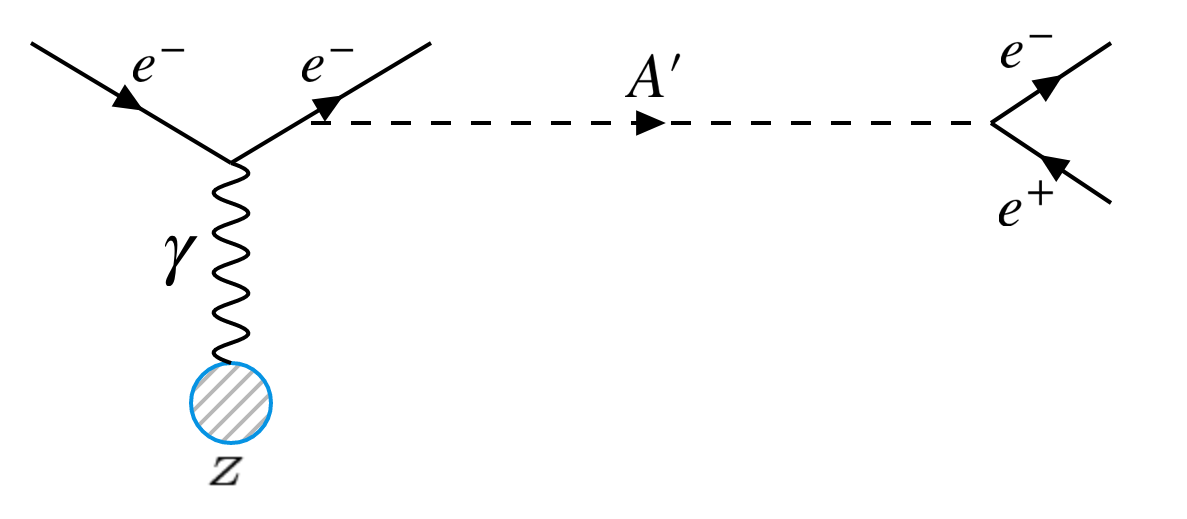
\includegraphics[width=14.5cm]{thesis_figures/VISIBLE.png}
\caption{Visible mode }
\label{fig:Visible_feynman}
\end{figure}

\begin{figure}[t!]
\centering
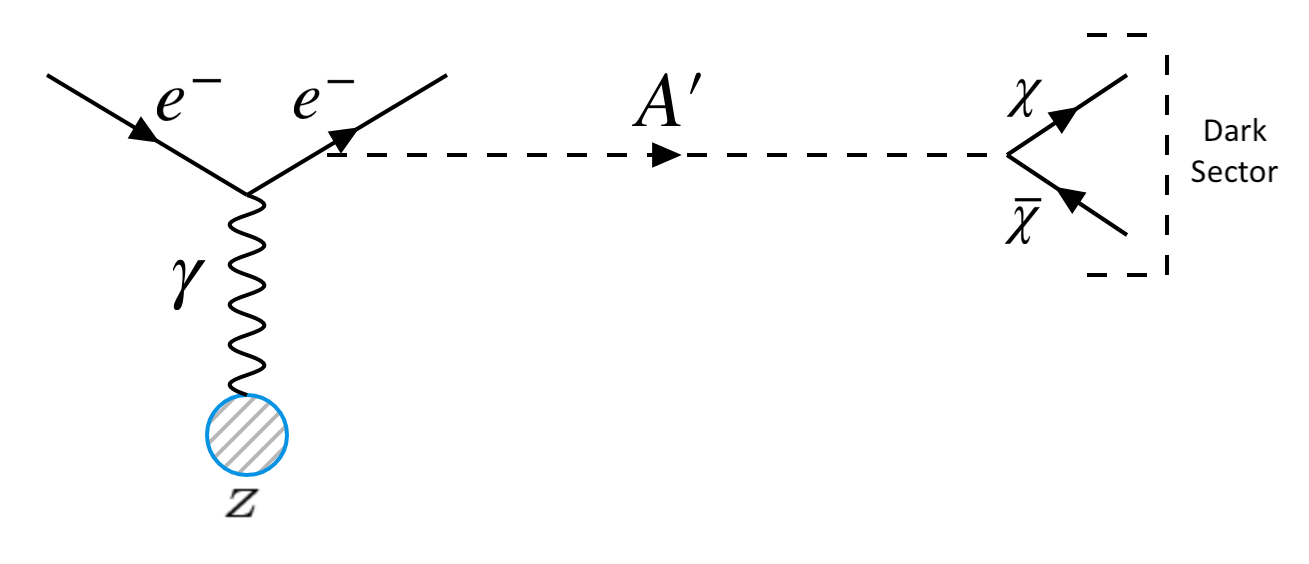
\includegraphics[width=15cm]{thesis_figures/INVISIBLE.png}
\caption{Invisible mode }
\label{fig:Invisible_feynman}
\end{figure}
Clearly from eq.(\ref{eq:Lagrangian}) there are two possibilities for the detection of $A'$. It can be either observed via its decay to SM particles which is called the \textit{visible mode} (fig.(\ref{fig:Visible_feynman})) or via its decay to light DM particles known as the \textit{invisible mode} (fig.(\ref{fig:Invisible_feynman})). In the visible mode we assume that $A'$ is one of the lightest states in the dark sector, then it is fair to believe that it would mainly decay to SM leptons. Such an interaction is described by the Lagrangian ${\cal L}_{int} = \epsilon e A'_{\mu} J^{\mu}_{em}$ where $J^{\mu}_{em}$ is the electromagnetic current and $e$ is the electromagnetic coupling. Such a decay would assume the $A'$ to have a sub-GeV mass and $\epsilon \ll 1 $. It also allows for an opportunity to set up an experiment for this particular mode since we will directly observe an excess of leptons in the final state. On the other hand for the invisible mode we assume that $A'$ is not the lightest state and there exists some other state $\chi$ with a lower mass, such that $A'\rightarrow \chi \overline{\chi}$ is a possibility. Such an event can also be probed with a so called missing energy experiment where the produced $A'$ or $\chi$ carries away some of the energy and is not detected.

The production and detection mechanisms discussed offer us the basic ingredients needed to set up an experiment for the detection of $A'$. One of the simpler layouts for such an experiment is an electron beam dump experiment. NA64 falls in this category, the setup of which is discussed in the next chapter.
\begin{figure}[t!]
\centering
  \begin{minipage}[t]{.45\textwidth}
    \centering
    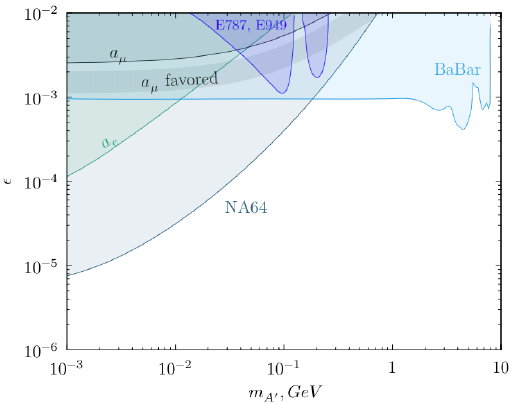
\includegraphics[width=\textwidth]{thesis_figures/exclusion_invisible.png}
    \caption{Current limits for invisible mode for 90\% C.L. exclusion region in the ($m_{A'},\epsilon$) plane ~\cite{2019EPJWC.21206005K}.}
    \label{fig:exclusion_invisible}
  \end{minipage}
  \hfill
  \begin{minipage}[t]{.45\textwidth}
    \centering
    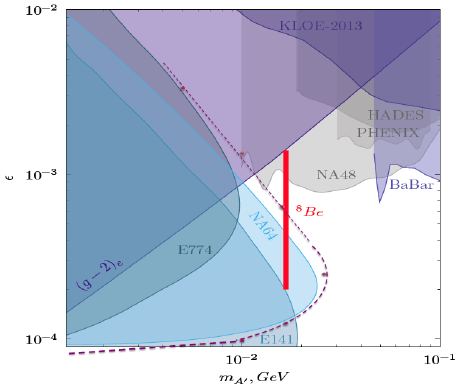
\includegraphics[width=\linewidth]{thesis_figures/exclusion_visible_latest.png}
    \caption{Current limits for invisible mode for 90\% C.L. exclusion region in the ($m_{A'},\epsilon$) plane. The blue plane is with 2017 data and the dotted line is with 2017+2018 data for NA64. The red line is the region that might explain the X17 boson~\cite{2019EPJWC.21206005K}.}
    \label{fig:exclusion_visible}
  \end{minipage}
\end{figure}


%%% Local Variables:
%%% mode: latex
%%% TeX-master: "mythesis"
%%% End:
